\documentclass[twocolumn,10pt]{article}
\usepackage{geometry}
\usepackage{mathptmx}
\usepackage{graphicx}
\usepackage{fancyhdr}
\usepackage{hyperref}
\usepackage{lastpage}
\geometry{
 a4paper,
 left = 0.625in,
 right = 0.625in,
 top = 1in,
 bottom = 1in
 }
\pagestyle{fancy}
\fancyhf{}
\rhead{CS648:Selected Topics in Network Algorithms}
\lhead{A course project report}
\cfoot{Page \thepage \hspace{1pt} of \pageref{LastPage}}
\date{}
\begin{document}
\title{\textbf{Switch Simulation for Performance Measurement}}
\author{Abhiram Singh, Sidharth Sharma\\Course Instructor: Prof. Ashwin Gumaste}
\maketitle
\thispagestyle{fancy}
\section{Introduction}
In current network scenario, end to end packet delay is measured as sum of propagation delay at each hop and processing delay at all intermediate switching devices.

Packet processing delay involves packet transmission delay and the time for which packet waits in the switch buffer (also known as queuing delay).
Buffers are provided because of the following reasons:
\begin{itemize}
\item To compensate the rate mismatch between transmission devices.
\item To handle bursty traffic.
\item To improve the link utilization.
\item To hold the packet until table look-up happen.
\item To hold the packet until destination port becomes free for transmission.
\end{itemize}
Buffers in the switch try to solve above mentioned problems but give rise to some other problems.

Out of mentioned three delays, propagation and transmission delay for a packet is fixed for a given path and transmission rate of each intermediate switch port.
However, queuing delay cannot be measured exactly for each packet because of the following reasons:
\begin{itemize}
\item Due to bursty traffic flow.
\item Due to behaviour of other flows is unknown.
\end{itemize}
Since queuing delay is the key deciding factor in providing Quality of Service in the network. Hence, it is necessary to observe its behaviour.

\section{Problem Description}
To observe the switch performance (throughput and port to port delay) with varying packet sizes. 

\section{Simulation Details}
For switch simulation, we used \textit{Simpy} discrete event simulation library in \textit{Python} .\\
Switch of 16 ports each of 10Gbps capacity is implemented.\\
Parameters of packets are defined in the class \textit{Packet}.

For traffic generation, \textit{PacketGenerator} class is defined which generates packets according to given packet size and generation rate.

Corresponding to each input port, input buffer is defined. Packet waits in the input buffer until it finds its output port in the switch based on the look-up.
\textit{Port} class defines the functionality of input buffer.

For each input buffer, there are 15 Virtual Output Queues(VoQ) corresponding to each output port.
Packet stays in the VoQ until the transmission of all the front packets in the VoQ is completed.
This wait depends on how many packets are in front of VoQ and how much contention each packet is experiencing from the VoQs associated with other input ports.
Code for VoQ is defined in the class \textit{VOQ}.

We attach a packet sink with the output ports in which all the packets are collected. This functionality is defined in the class \textit{PacketSink}.
To measure switch throughput, we defined \textit{SinkMonitor} class which periodically checks packet sink and update the throughput.

\section{Results}
We measured the throughput and port to port latency in the switch by varying packet sizes.
 
Delay vs packet size graph shows that on increasing packet size, port to port delay of the switch decreases. 
Reason behind this is more look-ups are required for smaller size packets in contrast to the larger size packets (less number of larger size packets are generated for the same data rate).
This result is shown in Figure \ref{Fig 1}.
\begin{figure}[h]
\centering
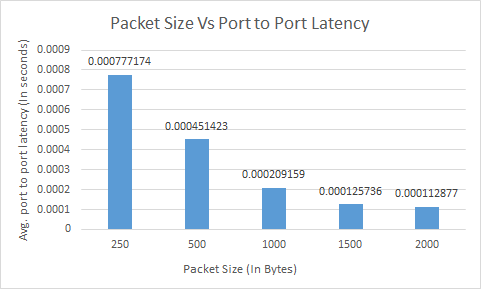
\includegraphics[width=0.95\linewidth]{latency.png}
\caption{Graph showing decrease in the port to port latency on increasing packet size.}
\label{Fig 1}
\end{figure}

On increasing average packet size we observed increase in throughput because port to port latency per packet for larger packet size is less.
This result is shown in Figure \ref{Fig 2}.
\begin{figure}[h]
\centering
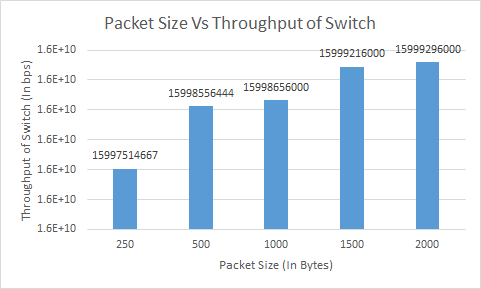
\includegraphics[width=0.95\linewidth]{throughput.png}
\caption{Graph showing increase in the switch throughput on increasing packet size.}
\label{Fig 2}
\end{figure}

\section{Conclusion}
The actual capacity of the switch varies with the average packet size of the flow. We observed the dependency of throughput and port to port latency of packet on average packet size of the flow.
Therefore, switch can be utilized in an efficient manner if larger average packet sizes are used in the flows.

\end{document}
